\section{Introduction}
Daily life assistance is one of the important missions for service robots. Especially, when the human tends to execute some tasks that are troublesome to perform alone due to the limitation in reachability or load, the humanoid robot that has a human-like body structure can be a great partner for the human (\figref{overview}). In this research, as the typical tasks where one needs other's help, we work on the manipulation tasks of both large rigid and flexible objects, and aim at the acquisition of the ability for humanoid robots to accomplish various manipulation tasks in cooperation with humans.\par
In the daily life environment, there are a wide variety of works needed to be done.
One of the difficulties in such cooperative works between a human and a robot is that the robot is expected to take actions autonomously according to what the human wants the robot to do.
In this research, we deal with this difficulty by decomposing cooperative works into local action generation and global transitions between those actions, and effectively utilizing multimodal information obtained from the cooperating human.

In the local action generation, we categorize the actions required in a series of cooperative tasks into three styles according to the attention target in the action, and realize each action by the imitation of human hand movement, walking velocity or arm posture taking advantage of the similarity in body structure and the feedback modification based on force and voice.

In the global transitions, the robot switches its motion at appropriate timing in proper order by detecting multimodal simple instructions from the human.

Using this framework, leaving the high order decisions in human hands and following the multimodal signs by the human, the robot can take an action that is autonomously acquired with the local purpose based on perceptual processing, and finally perform various cooperative tasks with the human co-worker.

\begin{figure}[htbp]
 \begin{center}
  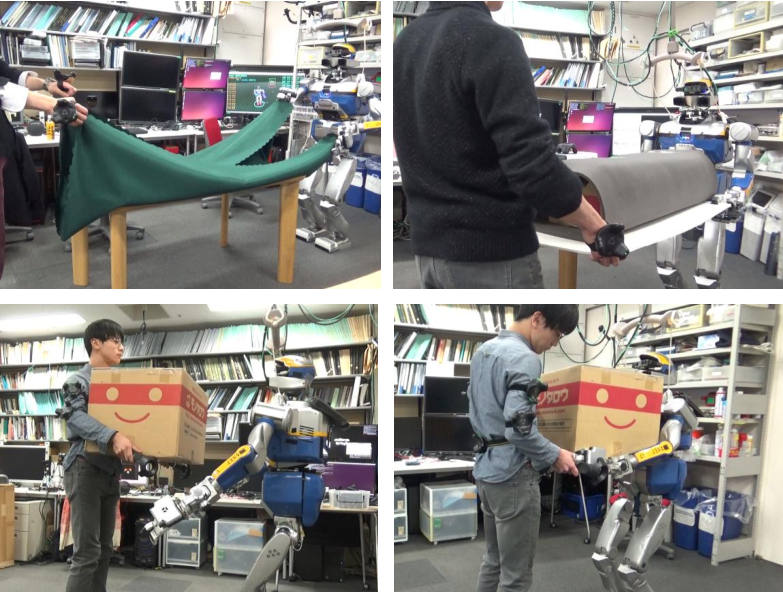
\includegraphics[width=1.00\columnwidth]{figs/several_tasks2}
  \caption{Several tasks dealt with in this paper; folding a large cloth, carrying a large board with other objects on it and passing large objects from a human to a robot.}
  \label{figure:overview}
 \end{center}
\end{figure}

\subsection{Related Works}

\subsubsection{Robot-robot Cooperative Works}
There are some researches on cooperative works by two robots~\cite{robot-robot1}\cite{robot-robot2}\cite{robot_robot_assmble}, not by a human and a robot. These researches are efficient if we consider the situation where the objective task has a fixed order between its included processes beforehand like a task in factories. However, under the household situations, the tasks don't necessarily come in the same order. Since it is difficult for a standalone robot to perform an advanced judgment like deciding the order of processes in order to execute the whole task or when to go on to the next process, programmers have to prepare the whole robot motions for each task when they want the robots to execute different tasks. It is not suitable for manipulation tasks in the daily life environment including several processes in several orders. In this research, assuming a household situation where there is a human in front of the robot, we solve such problems by relying on the human making those high-quality decisions. With the robot obeying the human requests, the objective tasks are executed.

\subsubsection{Human-robot Cooperative Works}
Human-robot cooperation can be seen in several types. Passing an relatively small item to a human who needs it will be one collaborative work~\cite{collaborative_primitives}\cite{handover_usage}. Wearable robots assisting humans are also in this field~\cite{wearable}\cite{exoskeleton}. Manipulating a single object with a human and a robot, transportation of a large panel or a table~\cite{aist_cooperative_carrying}\cite{carry_table} is also studied. However, although a certain task can be executed following these studies, these works are specialized and thus limited to a single certain task; passing an item, providing an extra hand or carrying a table. To achieve a series of tasks in the household situations, it is not enough and have to be integrated.
%% Since these studies are limited with the small size of the manipulated objects or the small areas where the robot end effector reaches, there are considerable needs that the robots can manipulate large objects in cooperation with humans.\par

On the other hand, when manipulating the same objects with two operators that are too large to be manipulated by one, communication and interaction between the two become more important than manipulating different things. The methodologies for communicating and interacting include voice recognition~\cite{voice_recognition}, visual gesture understanding~\cite{gesture}\cite{gesture2}\cite{task_analysis}, and also haptic (force/torque) information~\cite{aist_cooperative_carrying}\cite{carry_table}\cite{carry_with_vision}\cite{cooperative_nao} can be joined.

\subsubsection{Motion Acquirements by Imitation Learning}
There are a lot of attempts for robots to acquire deliberate actions by first imitating human motions and then learning the meaning of them~\cite{folding_dl}. The object of these studies is that the robot learns and gets a skill to accomplish a certain task on their own. However, not considering cooperativity, these learned actions are hard to be applied to cooperative works where the communication with each other is important. In this paper, we adopt a pure imitation of the human motion when deciding the robot motion, which is the simplest reaction in the field of imitation learning, but is the most basic and the most generic approach.

\subsection{Contributions and Overview of this Paper}

\begin{figure}[htbp]
 \begin{center}
  %% \includegraphics[width=0.80\columnwidth]{figs/nowprinting}
  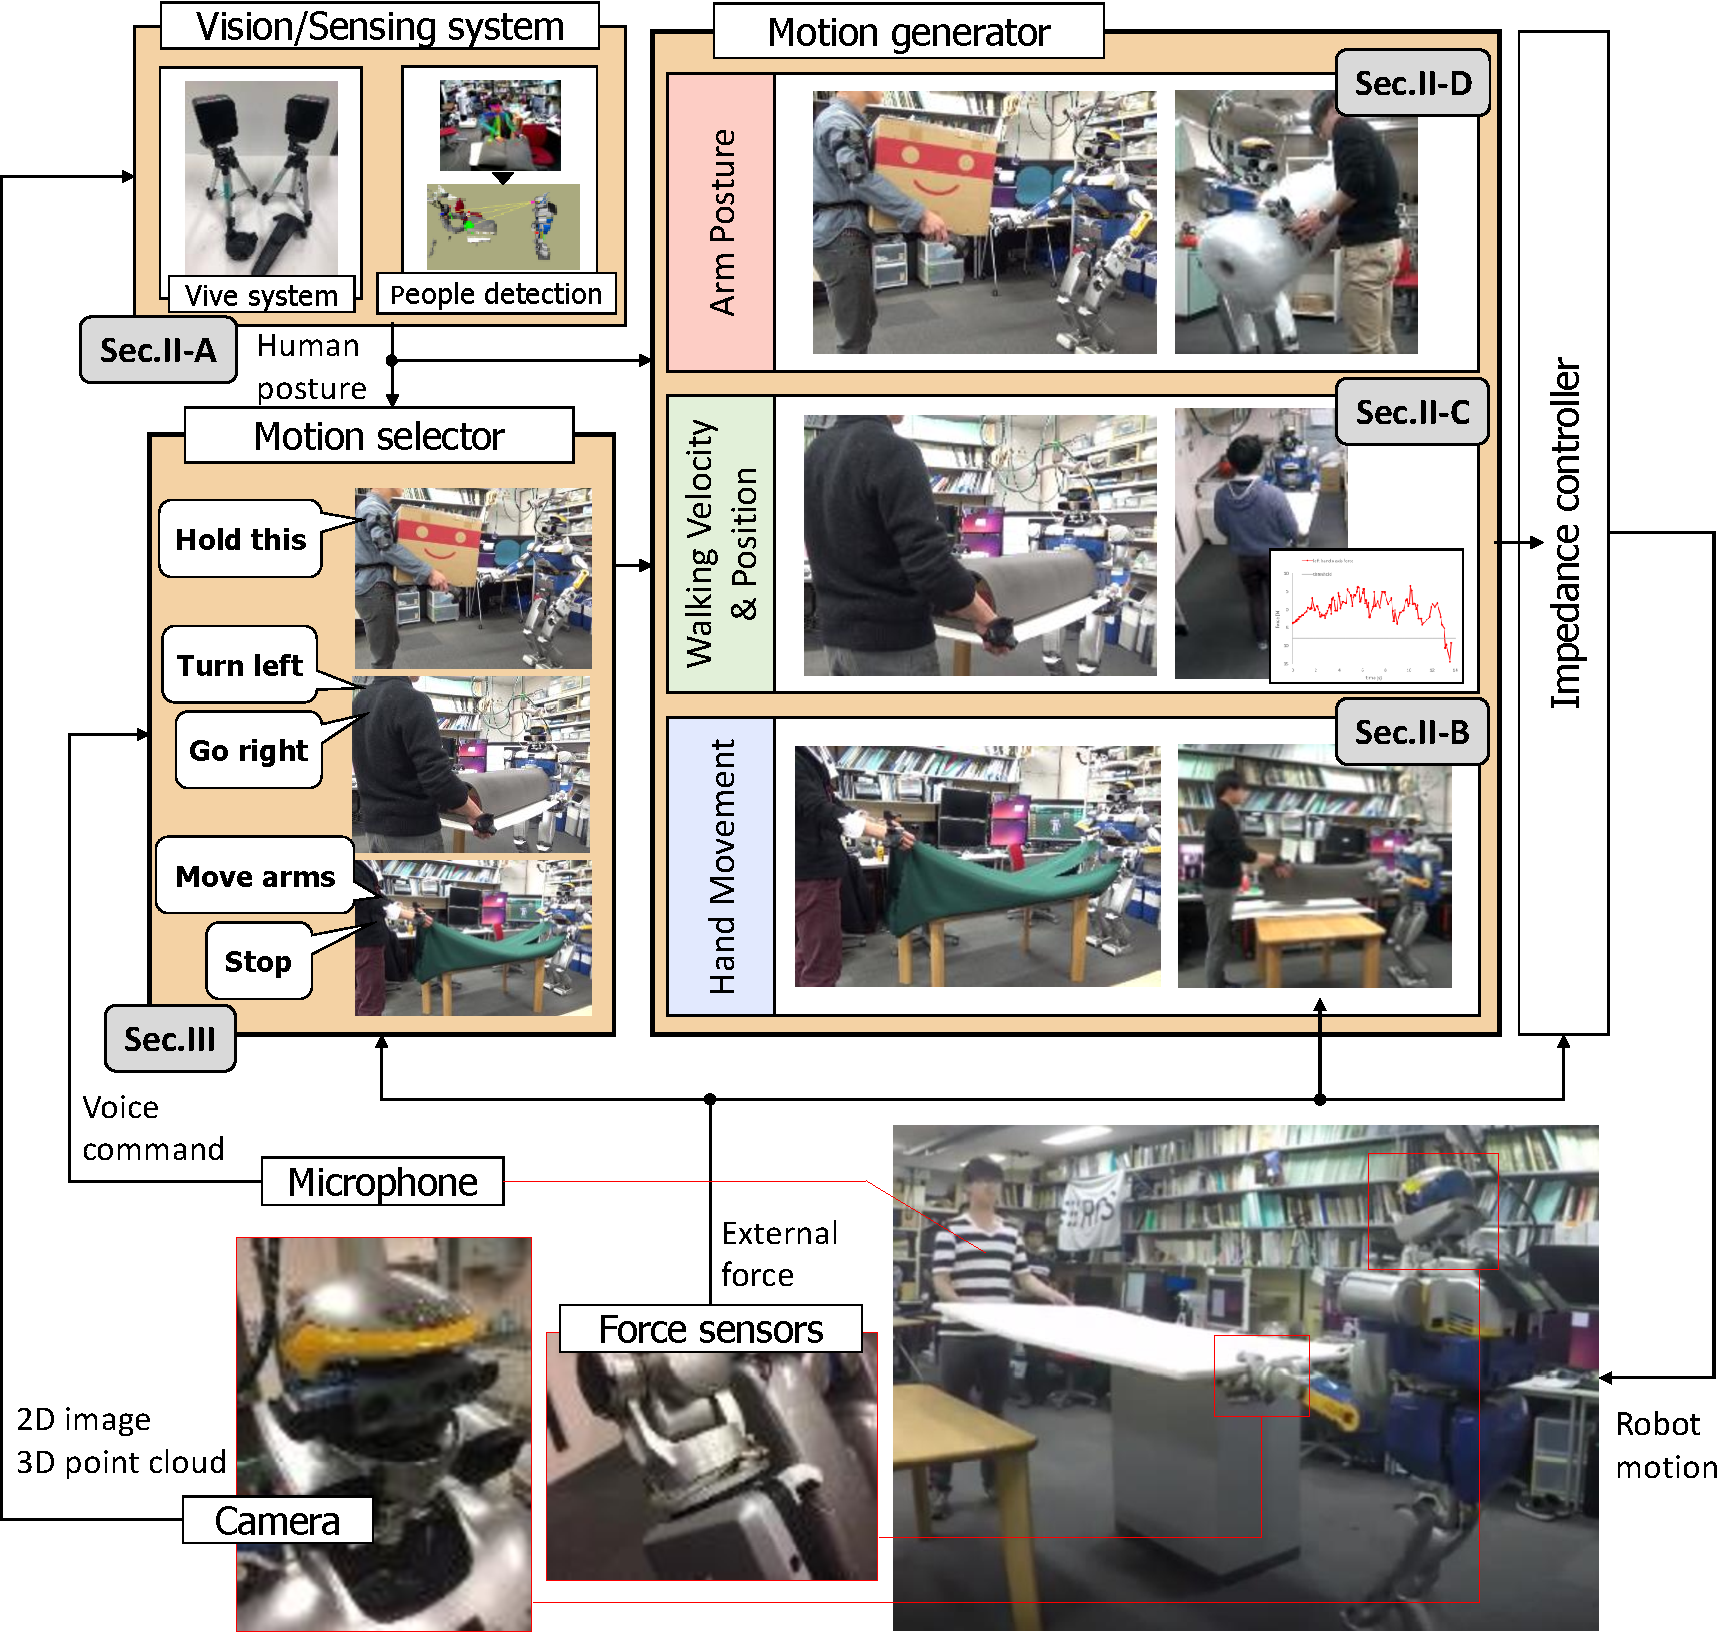
\includegraphics[width=1.00\columnwidth]{figs/all_system2}
  \caption{Proposed system in this paper.}
  \label{figure:system}
 \end{center}
\end{figure}

Here, we would like to discuss the requirements in the robots among the human-robot collaborative tasks manipulating one object at the same time. The robots
\begin{enumerate}
 \item need to acquire their motions adequate to achieve the purpose with helping humans,
 \item must realize 1) in a safety manner and meet the objects' constraints,
 \item should have a framework to obey the human commands sustainably.
\end{enumerate}
We take an approach to satisfy these needs by combining visual recognition, haptic information and speech interaction as shown in \figref{system}. First, the robot gets its motions observing human motions and imitating them. Here, we prepare a vision system to obtain human motion information. Then, referring force sensors data, those robot motions are modified to satisfy the objects' constraints. Finally, by introducing a speech recognition system, we constructed an integrated cooperative task executing system where a human can instruct the robot how to and when to take actions by aural communication.\par
In the following, we explain the methods how the robot gets its motion referring human motion in \secref{motion_generator}, and the integrated system for collaborative works based on those motions in \secref{aural}. Then, we show the experiments with the real robot applying the whole system in \secref{ex}.
